% !TeX root = statnicaEKT.tex
\part{BPC-KS1 - Komunikační Systémy 1}
\begin{huge}
	Otázky:
	\newline
\end{huge}
\begin{enumerate}
	\item Otázka - Zdrojové a kanálové kódování (komprese hlasu, zvuku, videa a dat, konvoluční a blokové kódy).
	\item Otázka - Analogové a digitální pásmové modulace (amplitudové, fázové, kmitočtové, QAM). 
	\item Otázka - Synchronizace. Obvody pro obnovu nosné vlny a časování symbolů, metody rámcové a síťové synchronizace. 
\end{enumerate}

%%%%%%%%%%%%%%%%%%%%%%%%%%%%%%%%%%%%%%%%%%%%%%%%%%%
\chapter{Zdrojové a kanálové kódovanie}
%%%%%%%%%%%%%%%%%%%%%%%%%%%%%%%%%%%%%%%%%%%%%%%%%%%

\section{Zdrojové kódovanie -- kompresia signálov}

Cieľom zdrojového kódovania je odstrániť z prenášaného signálu nadbytočné
informácie a znížiť tak potrebný dátový tok. Prezentácia rozlišuje dva pojmy:

\begin{itemize}
    \item \textbf{Redundancia} -- množstvo znakov alebo bitov, ktoré možno eliminovať bez
        straty užitočnej informácie. Jej odstránením vzniká \textit{bezstratová kompresia}.
        Príklady: ZIP, PNG, Huffmanov kód, LZW (Lempel--Ziv--Welch).
    \item \textbf{Irelevancia} -- nepodstatná zložka informácie, ktorú možno potlačiť pri
        zachovaní požadovanej kvality signálu. Jej odstránením vzniká \textit{stratová kompresia}.
        Príklady: MP3, JPEG (Joint Photographic Experts Group), MPEG (Moving Picture Experts Group).
\end{itemize}

\subsection{Kódovanie rečových signálov}

\subsubsection{PCM -- pulzná kódová modulácia (Pulse Code Modulation)}

PCM je základný spôsob prevodu analógového signálu do digitálnej podoby -- ide
o analógovo-digitálny (A/D) prevodník. Princíp pozostáva z troch krokov:

\begin{enumerate}
    \item \textbf{Vzorkovanie} -- signál sa meria v pravidelných intervaloch (pre hlas
        typicky 8\,000-krát za sekundu). Musí byť splnený Nyquistov--Shannonov
        teorém: vzorkovací kmitočet $f_s \geq 2f_m$, kde $f_m$ je najvyšší kmitočet
        v spektre signálu. Pri nesplnení dochádza k aliasingu -- prekryvu spektrálnych
        zložiek.
    \item \textbf{Kvantovanie} -- každý vzorek sa zaokrúhli na najbližšiu kvantovaciu
        úroveň. Pre $N$ bitov existuje $M = 2^N$ úrovní. Chyba zaokrúhlenia tvorí
        kvantovací šum, ktorého efektívna hodnota je $N_{RMS} = \Delta U / \sqrt{12}$.
        Každý pridaný bit zlepší odstup signál/šum SNR (Signal to Noise Ratio) o $6\,\mathrm{dB}$.
    \item \textbf{Kódovanie} -- každej úrovni sa priradí binárne číslo (pri 8 bitoch
        existuje 256 úrovní, čo zodpovedá dátovému toku 64\,kbit/s pre telefónny hlas).
\end{enumerate}

\begin{figure}[H]
    \centering
    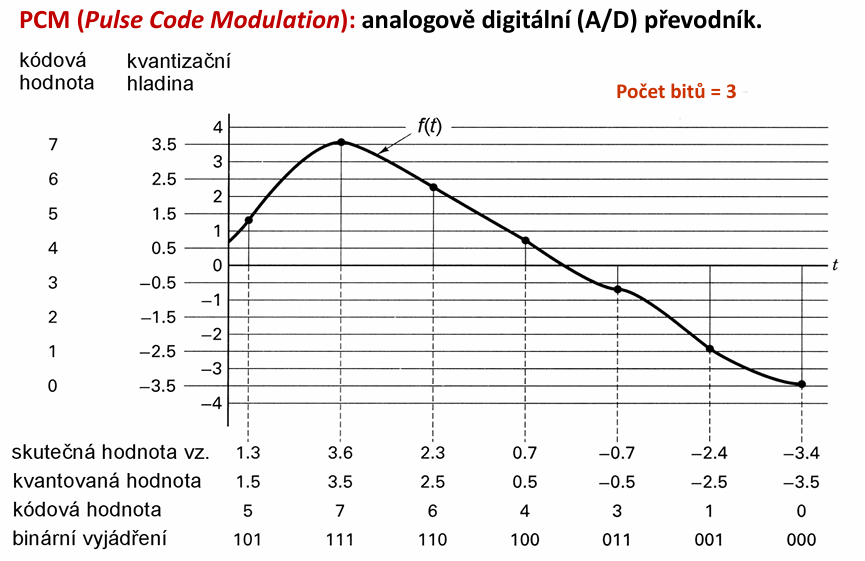
\includegraphics[width=0.85\textwidth]{Obrazky/Obrazky_KS1/fig_pcm_kvantovani.png}
    \caption{PCM -- lineárne kvantovanie. Vzorkovaný signál je priradený k najbližšej
    kvantovacej úrovni. Pre 3 bity existuje 8 úrovní. Kvantovací šum vzniká
    rozdielom skutočnej a kvantovanej hodnoty.}
    \label{fig:pcm}
\end{figure}

\textbf{Lineárne vs. nelineárne kvantovanie:} V ľudskej reči prevládajú nízke
hlasitosti -- veľké amplitúdy sú málo časté. Pri lineárnom kvantovaní by úseky s
malou amplitúdou boli kvantované s veľkou relatívnou chybou. Preto sa v praxi
(telefónia) používa \textbf{nelineárne kvantovanie} (A-law v Európe, $\mu$-law v
USA): pri malých amplitúdach sú kvantizačné kroky jemné (je ich viac), pri veľkých
hrubé (je ich menej). Výsledkom je rovnaká subjektívna kvalita pri menšom počte
bitov.

\subsubsection{DPCM -- diferenčná pulzná kódová modulácia (Differential Pulse Code Modulation)}

Susedné vzorky rečového signálu sú si veľmi podobné, pretože rečový signál je
časovo korelovaný. Namiesto absolútnej hodnoty vzorku sa preto prenáša \textbf{iba
rozdiel medzi skutočnou hodnotou a hodnotou predikovanou} z predchádzajúcich vzorkov.

\begin{figure}[H]
    \centering
    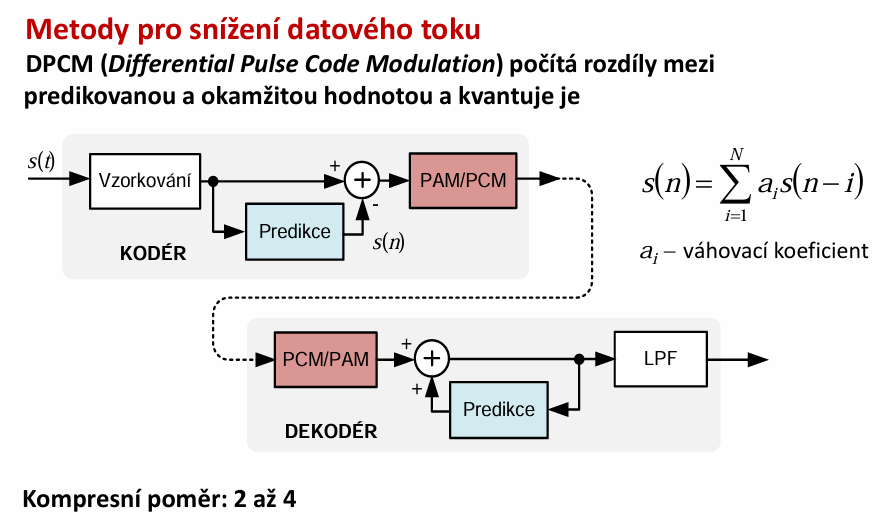
\includegraphics[width=0.80\textwidth]{Obrazky/Obrazky_KS1/fig_dpcm.png}
    \caption{Blokové schéma DPCM kodéra (hore) a dekodéra (dole). Kodér vypočíta
    rozdiel medzi skutočnou a predikovanou hodnotou vzorku a tento (malý) rozdiel
    prenáša. Dekodér pripočíta prijatý rozdiel k vlastnej predikcii a rekonštruuje
    signál.}
    \label{fig:dpcm}
\end{figure}

Prenáša sa iba predikčná chyba, ktorá má typicky malý rozptyl -- na jej zakódovanie
stačí menej bitov. Dosiahnuteľný \textbf{kompresný pomer je 2 až 4} oproti PCM.

\subsubsection{Vokodér -- parametrické kódovanie hlasu}

Vokodér nevysiela tvar zvukového signálu, ale \textbf{parametre modelu ľudského
hlasového traktu}. Vychádza z anatómie: znelé hlásky vznikajú periodickými impulzmi
hlasiviek (glottis), neznelé hlásky šumovým signálom z úst -- oba budiace signály
prechádzajú cez hlasový trakt (krk, ústa, nos), ktorý funguje ako filter.

\begin{figure}[H]
    \centering
    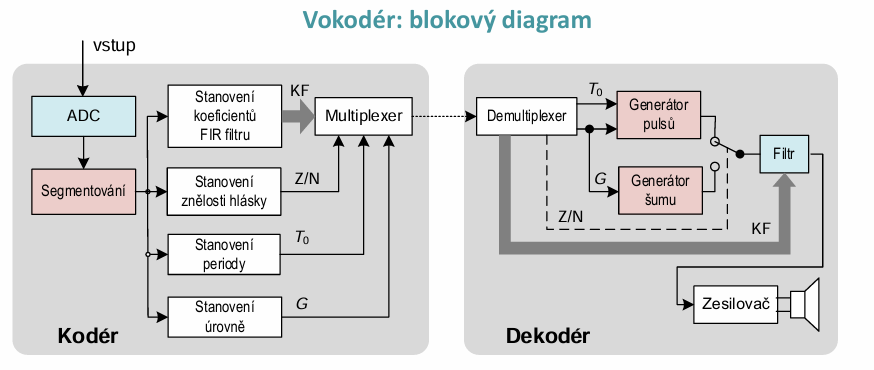
\includegraphics[width=0.85\textwidth]{Obrazky/Obrazky_KS1/fig_vokoder.png}
    \caption{Blokové schéma vokodéra. Kodér analyzuje reč po krátkych úsekoch
    (10--30\,ms -- parametre hlasového traktu sú v tomto úseku konštantné) a
    určuje: koeficienty filtra (KF), znelosť/neznelosť hlásky (Z/N), periódu
    základného tónu ($T_0$) a hlasitosť ($G$). Tieto parametre sa prenášajú.
    Dekodér budením príslušného generátora cez syntetický filter rekonštruuje reč.}
    \label{fig:vokoder}
\end{figure}

Namiesto tisícov vzorkov signálu sa prenáša iba niekoľko parametrov každých
20\,ms. Kvalita syntetizovanej reči je nižšia, ale dátový tok môže byť veľmi malý
(pod 4\,kbit/s).

\textbf{CELP} (Code Excited Linear Prediction -- lineárna predikcia s kódovým
budením): moderná varianta -- budený signál sa vyberá z vopred uloženého slovníka
(codebook) excitačných vektorov. Prenáša sa iba adresa (index) najlepšieho vektora.
Dosahuje rýchlosť 4\,kbit/s a menej. Používa sa v mobilných sieťach GSM (Global
System for Mobile Communications) a 3G.

\subsubsection{MPEG -- kódovanie zvuku}

MP3 a ostatné formáty MPEG využívajú \textbf{psychoakustický model} -- vlastnosti
ľudského sluchu:

\begin{itemize}
    \item \textbf{Kmitočtové maskovanie}: silný tón na určitom kmitočte maskuje slabšie
        tóny vo svojom frekvenčnom okolí -- tie sa stávajú pre poslucháča nepočuteľnými.
        Kmitočtové maskovacie krivky určujú, ako dielčie čisté tóny maskujú zvuky
        v ich okolí.
    \item \textbf{Časové maskovanie}: silný zvuk saturuje receptory vo vnútornom uchu
        a je potrebná určitá doba pre obnovenie ich činnosti -- zvuky bezprostredne
        pred a po hlasnom zvuku sú ťažšie rozoznateľné.
    \item Zložky signálu pod prahom sluchu sú nevnímateľné a neprenášajú sa.
\end{itemize}

Postup kódovania MPEG: signál sa rozdelí bankou filtrov do 32 subpásiem, pomocou
psychoakustického modelu sa určia maskovacie úrovne v každom subpásme a každému
pásmu sa pridelí zodpovedajúci počet bitov. Výsledok: subjektívne kvalitný zvuk
pri dátovom toku 128--320\,kbit/s namiesto 1\,411\,kbit/s pri CD.

\subsection{Kódovanie obrazu a videa}

\begin{itemize}
    \item \textbf{JPEG} (Joint Photographic Experts Group) -- transformačné kódovanie
        pre statické obrazy. Každý snímok sa rozdelí na bloky 8$\times$8 pixelov.
        Každý blok sa transformuje diskrétnou kosínusovou transformáciou DCT
        (Discrete Cosine Transform) do frekvenčnej oblasti a koeficienty zodpovedajúce
        vyšším priestorovým frekvenciám, ktoré sú pre ľudské oko menej dôležité,
        sa kvantujú hrubo alebo zahodia. Stratová kompresia fotografií.
    \item \textbf{MPEG} (Moving Picture Experts Group) -- hybridné kódovanie (DCT +
        prediktívne + vektory pohybu) pre pohyblivé obrazy. Navyše využíva
        \textit{časovú redundanciu}: po sebe idúce snímky videa sú si podobné.
        Prenášajú sa iba \textit{rozdiely} medzi snímkami a \textit{vektory pohybu}
        popisujúce posun objektov. Základ filmov, DVB (Digital Video Broadcasting),
        Blu-ray.
\end{itemize}

\subsection{Bezstratová kompresia dát}

\begin{itemize}
    \item \textbf{Huffmanov kód} -- neadaptívne kódovanie s preddefinovaným slovníkom.
        Symboly s vyššou pravdepodobnosťou výskytu dostávajú kratšie kódové slová,
        symboly s nižšou pravdepodobnosťou dlhšie. Priemerná dĺžka kódového slova
        sa tak minimalizuje.
    \item \textbf{LZW} (Lempel--Ziv--Welch) -- adaptívny slovníkový algoritmus
        s dynamicky vytváraným slovníkom. Hľadá opakujúce sa reťazce v dátach
        a nahrádza ich krátkymi kódmi. Používa sa v GIF, ZIP, ARJ.
\end{itemize}

%%%%%%%%%%%%%%%%%%%%%%%%%%%%%%%%%%%%%%%%%%%%%%%%%%%
\section{Kanálové kódovanie -- blokové a konvolucné kódy}
%%%%%%%%%%%%%%%%%%%%%%%%%%%%%%%%%%%%%%%%%%%%%%%%%%%

\section{Prečo kanálové kódovanie?}

Kanálové kódovanie zvyšuje odolnosť signálu proti chybám vznikajúcim pri prenose
komunikačným kanálom (vplyvom aditivného rušenia, medzisymbolových preslechov,
úniku signálu). Riešením je pridanie \textbf{zabezpečovacích (redundantných) bitov}
k prenášanej správe. Tieto bity umožnia prijímaču:
\begin{itemize}
    \item \textbf{Detegovať} chyby -- rozpoznať, že prijaté slovo nezodpovedá žiadnemu
        platnému kódovému slovu.
    \item \textbf{Opraviť} chyby bez nutnosti opakovania prenosu -- FEC (Forward Error
        Correction -- dopredná korekcia chýb).
\end{itemize}

Alternatívou je \textbf{ARQ} (Automatic Repeat reQuest -- automatická žiadosť
o opakovanie): detekcia chýb s požiadavkou na opakovanie chybného bloku. Vyžaduje
spätný kanál.

\textbf{Kódový pomer} $R = k/n$ udáva pomer počtu informačných bitov $k$ k
celkovému počtu bitov kódového slova $n$.

\subsection{Kľúčový pojem: Hammingova vzdialenosť}

\textbf{Hammingova vzdialenosť} $d(u, v)$ dvoch binárnych slov je počet pozícií,
v ktorých sa líšia. Napríklad pre $u = 10010$ a $v = 01011$ platí $d(u,v) = 3$.

\textbf{Minimálna Hammingova vzdialenosť} $d_{min}$ je najmenšia hodnota vzdialenosti
medzi všetkými kódovými slovami kódu. Určuje opravné schopnosti:
\begin{itemize}
    \item Maximálny zaručený počet detegovateľných chýb: $k_z = d_{min} - 1$
    \item Maximálny zaručený počet opraviteľných chýb: $k_o = \lfloor(d_{min}-1)/2\rfloor$
\end{itemize}

\subsection{Paritný kód -- najjednoduchší blokový kód}

K prenášanému slovu sa pridá jeden \textbf{paritný bit} tak, aby celkový počet
jednotiek bol párny (sudá parita). Prijímač skontroluje paritu -- ak je nepárna,
nastala chyba. Kód má $d_{min} = 2$, teda deteguje jednonásobné chyby, ale
nedokáže ich opraviť.

\textbf{Iteračný (súčinový) kód}: dáta sa usporiadajú do matice a paritné bity
sa počítajú pre každý riadok aj každý stĺpec. Umožňuje nielen detegovať, ale aj
\textbf{lokalizovať a opraviť} jednonásobnú chybu -- prienik chybného riadka a
chybného stĺpca jednoznačne určí pozíciu chybného bitu.

\subsection{Lineárne blokové kódy}

Lineárny blokový kód $(n, k)$ zobrazuje blok $k$ informačných bitov na kódové
slovo dĺžky $n$ bitov, pričom $n - k$ bitov tvorí zabezpečovaciu časť.

Kódovanie sa vykonáva pomocou \textbf{generujúcej matice} $\mathbf{G}$:
zabezpečovacie bity sú lineárnymi kombináciami (XOR -- eXclusive OR, exkluzívny
súčet) vybraných informačných bitov, každý kontroluje inú podmnožinu.

V prijímači sa vypočíta \textbf{syndróm} $\mathbf{s} = \mathbf{r} \cdot \mathbf{H}^T$,
kde $\mathbf{H}$ je kontrolná matica. Syndróm rovný nule indikuje bezchybný príjem;
nenulový syndróm jednoznačne určuje pozíciu chyby.

\subsection{Hammingove kódy}

Hammingove kódy sú lineárne kódy s $d_{min} = 3$, kde \textbf{binárna hodnota
syndrómu priamo udáva pozíciu chybného bitu} -- nie je potrebné žiadne vyhľadávanie
v tabuľke chýb.

Štruktúra kódu: k 4 informačným bitom sa pridajú 3 zabezpečovacie bity $\Rightarrow$
kód (7,4), $R = 4/7$. Zabezpečovacie bity sú umiestnené na pozíciách mocnín čísla
2 (1, 2, 4) a každý kontroluje iné podmnožiny bitov kódového slova.

\begin{figure}[H]
    \centering
    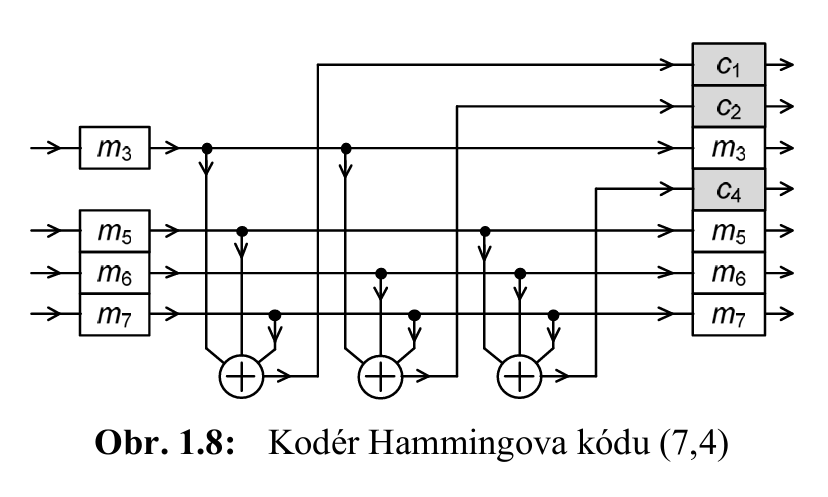
\includegraphics[width=0.65\textwidth]{Obrazky/Obrazky_KS1/fig_hamming_koder.png}
    \caption{Kodér Hammingovho kódu (7,4). Hradlá XOR počítajú kontrolné bity
    $c_1$, $c_2$, $c_4$ zo zdrojových bitov $m_3, m_5, m_6, m_7$. Výsledné
    kódové slovo: $[c_1\, c_2\, m_3\, c_4\, m_5\, m_6\, m_7]$.}
    \label{fig:hamming_koder}
\end{figure}

\begin{figure}[H]
    \centering
    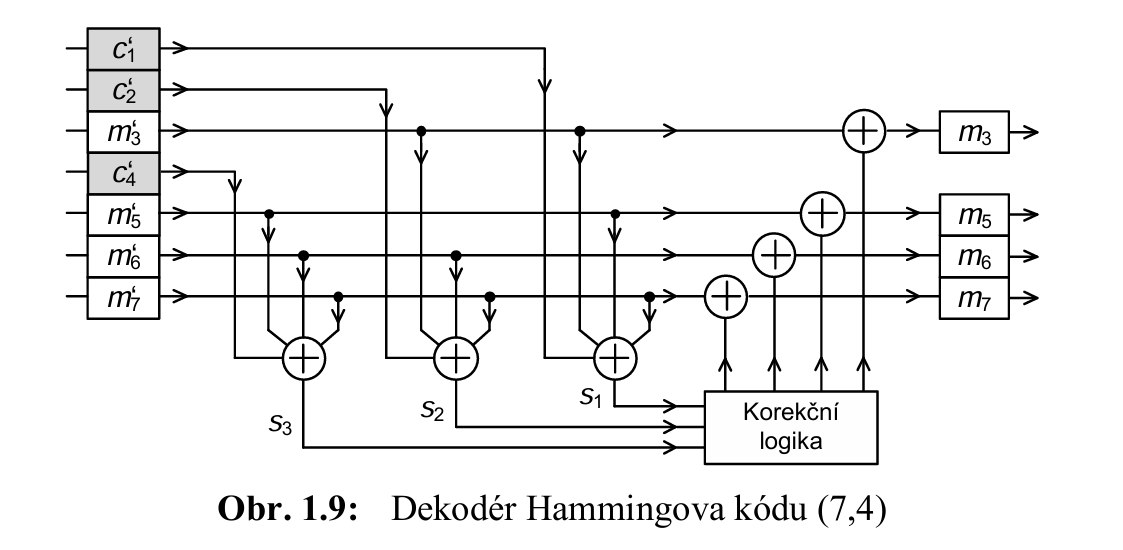
\includegraphics[width=0.65\textwidth]{Obrazky/Obrazky_KS1/fig_hamming_dekoder.png}
    \caption{Dekodér Hammingovho kódu (7,4). Syndróm $[s_3\, s_2\, s_1]$ sa
    vypočíta z prijatého slova. Jeho binárna hodnota priamo zodpovedá pozícii
    chybného bitu (napr. syndróm $= 101_2 = 5 \Rightarrow$ chyba na 5. pozícii).
    Korekčná logika bit invertuje.}
    \label{fig:hamming_dekoder}
\end{figure}

Príklady: HK(7,4), HK(15,11), HK(31,26). Opravujú jednonásobné chyby ($t=1$).
Rozšírený Hammingov kód (pridanie globálneho paritného bitu) má $d_{min} = 4$:
opravuje jednonásobné a deteguje dvojnásobné chyby.

\subsection{Cyklické kódy}

Cyklické kódy sú špeciálne lineárne kódy s vlastnosťou: \textbf{cyklickým posunom
ľubovoľného kódového slova vznikne opäť platné kódové slovo}. Táto algebraická
štruktúra umožňuje implementovať kodéry a dekodéry pomocou jednoduchých posuvných
registrov so spätnou väzbou.

\textbf{CRC} (Cyclic Redundancy Check -- cyklická kontrola redundanciou) --
najpoužívanejší cyklický kód na detekciu chýb. Zabezpečovacie bity sa vypočítajú
ako zvyšok po delení polynomiálnou reprezentáciou dát generujúcim polynómom $g(x)$.
Prijímač overí, či je zvyšok nulový. Používa sa v Ethernete, USB (Universal Serial
Bus), ZIP, UART (Universal Asynchronous Receiver-Transmitter).

\textbf{BCH} (Bose--Chaudhuri--Hocquenghem) \textbf{a Reed-Solomonove kódy} --
pokročilejšie cyklické kódy schopné opravovať viac chýb ($t > 1$). Reed-Solomon
pracuje so symbolmi (skupinami bitov) a je obzvlášť účinný pri oprave
\textit{zhlukov chýb} -- používa sa v CD, DVD, QR kódoch a satelitnej komunikácii.

\subsection{Konvolucné kódy}

Konvolucné kodéry spracúvajú vstupnú postupnosť \textbf{kontinuálne} -- na rozdiel
od blokových kódov nepracujú s blokmi pevnej dĺžky. Každý výstupný bit je lineárnou
kombináciou (XOR) aktuálneho vstupného bitu a niekoľkých predchádzajúcich bitov
uchovaných v posuvnom registri (pamäť kodéra dĺžky $m$).

Parametre kódu: dĺžka bloku výstupného slova $n_0$, dĺžka bloku správy $k_0$,
kódový pomer $R = k_0/n_0$, dĺžka kódového obmedzenia $mk_0$.

\begin{figure}[H]
    \centering
    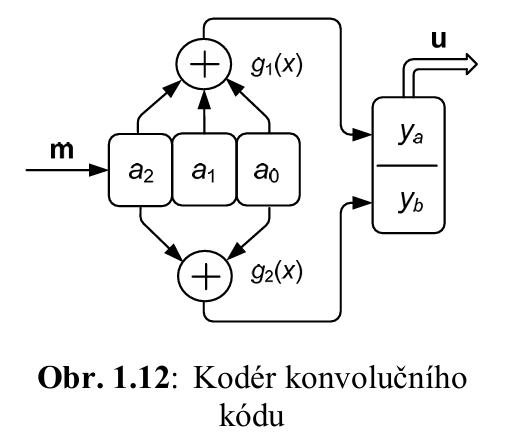
\includegraphics[width=0.50\textwidth]{Obrazky/Obrazky_KS1/fig_konvolucni_koder.png}
    \caption{Kodér konvolucného kódu s kódovým pomerom $R=1/2$ a dĺžkou pamäte
    $K=3$. Posuvný register uchováva aktuálny a dva predchádzajúce vstupné bity.
    Pre každý vstupný bit sa vygenerujú dva výstupné bity ako rôzne XOR kombinácie
    obsahu registra.}
    \label{fig:konv_koder}
\end{figure}

\textbf{Mriežkový (trellis) diagram} je grafická reprezentácia všetkých možných
stavových prechodov kodéra. Každý uzol reprezentuje stav posuvného registra,
každá hrana zodpovedá jednému vstupnému bitu a je označená zodpovedajúcimi
výstupnými bitmi. Pre vstupnú postupnosť dĺžky $L$ existuje na $L$-tej úrovni
stromu $2^L$ rozvetvení, ale iba $2^m$ rôznych stavov -- preto sa prechádza na
mriežkový diagram.

\begin{figure}[H]
    \centering
    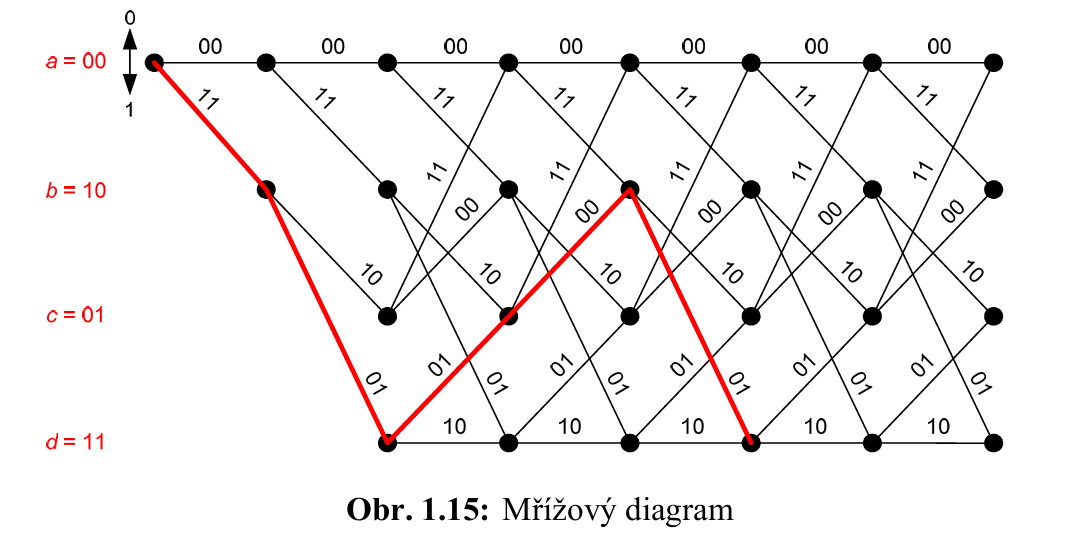
\includegraphics[width=0.80\textwidth]{Obrazky/Obrazky_KS1/fig_trellis.png}
    \caption{Mriežkový (trellis) diagram konvolucného kodéra s $K=3$. Štyri uzly
    zodpovedajú stavom posuvného registra (00, 10, 01, 11). Horné vetvy = vstupný
    bit 0, dolné vetvy = vstupný bit 1. Kódovanie správy
    $\mathbf{m}=[1\,1\,0\,1\,1]$ = tučne vyznačená cesta diagramom.}
    \label{fig:trellis}
\end{figure}

\subsubsection{Viterbiho algoritmus -- dekódovanie konvolucných kódov}

Viterbiho dekódovanie je optimálne dekódovanie s maximálnou vierohodnosťou
(ML -- Maximum Likelihood decoding) -- porovnávanie prijatej, chybami narušenej
postupnosti so všetkými postupnosťami, ktoré mohli byť vyslané.

\textbf{Viterbiho algoritmus} využíva princíp dynamického programovania:
\begin{enumerate}
    \item V každom časovom kroku sa vypočíta Hammingova vzdialenosť prijatého
        bloku dĺžky $n_0$ od všetkých možných blokov na každej vetve diagramu.
    \item Kumulovaná metrika (súčet vzdialeností) každej cesty sa priebežne
        aktualizuje.
    \item V rámci okna konečnej dĺžky sa v každom uzle zachová iba
        \textbf{prežívajúca cesta} (survivor path) -- tá s najmenšou kumulovanou
        metrikou; ostatné cesty sa eliminujú.
    \item Na konci sa vyberie cesta s minimálnou celkovou metrikou -- tá
        zodpovedá dekódovanej správe.
\end{enumerate}

\begin{figure}[H]
    \centering
    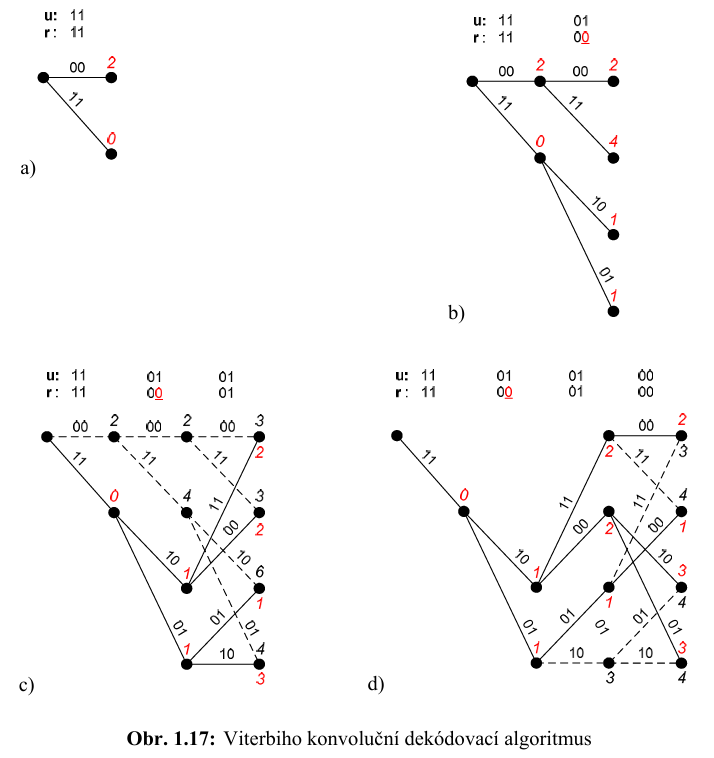
\includegraphics[width=0.85\textwidth]{Obrazky/Obrazky_KS1/fig_viterbi.png}
    \caption{Viterbiho dekódovací algoritmus -- kroky a) až d). Čísla pri uzloch
    sú kumulované Hammingove vzdialenosti (metriky ciest). V každom kroku sa
    eliminujú cesty s vyššou metrikou (prerušované čiary). Nakoniec zostane
    jediná optimálna cesta.}
    \label{fig:viterbi}
\end{figure}

\textbf{Tvrdé vs. mäkké rozhodovanie:}
\begin{itemize}
    \item \textbf{Tvrdé rozhodovanie} (hard decision): demodulátor kvantuje každý
        prijatý symbol na 0 alebo 1. Metrikou vetvy je Hammingova vzdialenosť.
        Jednoduché, ale vedie k strate informácie o spoľahlivosti rozhodnutia.
    \item \textbf{Mäkké rozhodovanie} (soft decision): demodulátor odovzdá dekodéru
        nekvantované hodnoty. Metrikou vetvy je euklidovská vzdialenosť. Zlepšenie
        oproti tvrdému rozhodovaniu je približne 2--3\,dB.
\end{itemize}

\textbf{Turbokódy}: dva konvolucné kodéry zapojené paralelne s prekladačom
(interleaverom) medzi nimi. Iteračné turbo dekódovanie s výmenou extrinsických
informácií medzi dekodérmi dosahuje výkon veľmi blízky Shannonovmu limitu kapacity
kanála. Používajú sa v LTE (Long Term Evolution, 4G).

%%%%%%%%%%%%%%%%%%%%%%%%%%%%%%%%%%%%%%%%%%%%%%%%%%%
\chapter{Analógové a digitálne pásmové modulácie}
%%%%%%%%%%%%%%%%%%%%%%%%%%%%%%%%%%%%%%%%%%%%%%%%%%%

\section{Prečo modulácia?}

Signál základného pásma moduluje sínusový priebeh -- \textbf{nosnú vlnu} -- tak,
aby zodpovedal charakteristikám prenosového kanálu. Nosná sa prevádza na
elektromagnetické pole (EM pole) za účelom šírenia na požadované miesto určenia
pomocou antén.

Klasifikácia modulácií:
\begin{itemize}
    \item Analógové (AM, FM, PM, QAM) vs. digitálne (ASK, FSK, PSK, QAM)
    \item Lineárne (s premennou modulačnou obálkou): AM (Amplitude Modulation),
        QAM (Quadrature Amplitude Modulation), ASK (Amplitude Shift Keying)
    \item Nelineárne (s konštantnou modulačnou obálkou): FM (Frequency Modulation),
        PM (Phase Modulation), FSK (Frequency Shift Keying), PSK (Phase Shift Keying)
    \item Koherentné (demodulácia s pomocou obnovenej nosnej): ASK, FSK, PSK
    \item Nekoherentné (demodulácia bez obnovenej nosnej): DPSK (Differential PSK),
        FSK, ASK
\end{itemize}

Harmonický signál $s_0(t) = S_0\cos(2\pi f_c t + \varphi_0)$ má tri parametre,
ktoré možno modulovať: amplitúdu $S_0$ (AM, ASK), kmitočet $f_c$ (FM, FSK)
a fázu $\varphi_0$ (PM, PSK).

\section{Amplitúdové modulácie}

\subsection{AM -- amplitúdová modulácia (Amplitude Modulation)}

Typické aplikácie: rozhlasové vysielanie na dlhých LW (Long Wave), stredných MW
(Medium Wave) a krátkych SW (Short Wave) vlnách (kmitočty od stoviek kHz do
jednotiek MHz) pri výkonoch v stovkách kW.

Amplitúda nosnej je lineárnou funkciou modulačného signálu. Obálka AM signálu:
$S(t) = S_0 + \Delta S \cdot n(t)$, kde $m = \Delta S / S_0$ je \textbf{hĺbka
modulácie} (typicky sa udáva v percentách, $0 < m \leq 1$) a $n(t)$ je normovaná
modulačná funkcia.

Spektrum AM signálu obsahuje tri zložky: nosnú na $f_c$ a dve postranné pásma
na $f_c \pm F$ (kde $F$ je kmitočet modulačného signálu).

\textbf{Výhoda AM}: jednoduchá asynchrónna demodulácia obálkovým demodulátorem
(dióda + RC článok) -- nevyžaduje obnovu nosnej.

\textbf{Hlavná nevýhoda AM}: je energeticky neefektívna. Vysielač musí byť
dimenzovaný na špičkový výkon $P_{PEP} = 4P_0$ (pri $m = 1$), pritom modulačná
účinnosť je len $\eta = 33\,\%$ -- nosná nenesie informáciu, ale spotrebuje
väčšinu výkonu.

\begin{figure}[H]
    \centering
    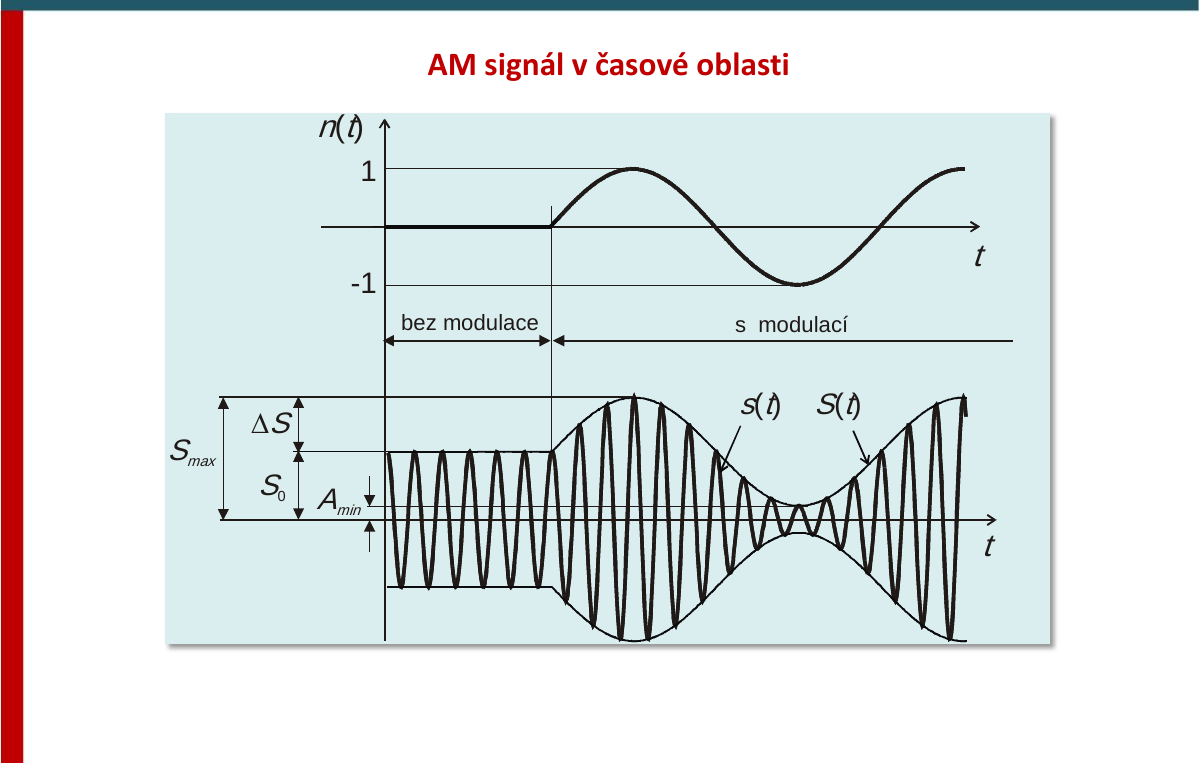
\includegraphics[width=0.88\textwidth]{Obrazky/Obrazky_KS1/fig_am_casova_oblast.png}
    \caption{AM signál v časovej oblasti. Hore: normovaný modulačný signál $n(t)$.
    Dole: AM signál $s(t)$ s obálkou $S(t)$. Bez modulácie má nosná konštantnú
    amplitúdu $S_0$; po zapnutí modulácie sa amplitúda mení od $A_{min} = S_0(1-m)$
    do $S_{max} = S_0(1+m)$ podľa modulačného signálu. Amplitudový zdvih je
    $\Delta S = mS_0$.}
    \label{fig:am_casova}
\end{figure}

\subsection{DSB -- obidve postranné pásma s potlačenou nosnou (Double Side Band -- Suppressed Carrier)}

Nosná zložka je potlačená -- \textbf{modulačná účinnosť je 100\,\%}, všetok
výkon je sústredený v postranných pásmach nesúcich informáciu. Demodulácia
vyžaduje koherentnú referenciu -- obnovu nosnej vlny v prijímači (umocňujúca
slučka, Costasova slučka).

\subsection{SSB -- jedno postranné pásmo (Single Side Band)}

Obidve postranné pásma DSB obsahujú tú istú informáciu -- prenáša sa iba jedno z
nich. SSB má \textbf{polovičnú šírku pásma} oproti DSB.

Výhody: maximálna spektrálna efektívnosť, väčší dosah pri rovnakom výkone.
Nevýhody: zložitejší modulátor (fázová metóda alebo filtrová metóda) a nutnosť
koherentnej demodulácie. Používa sa na krátkych vlnách (rádioamatéri, letecká
komunikácia).

\subsection{VSB -- vestigiálne postranné pásmo (Vestigial Side Band)}

Kompromis medzi DSB a SSB. Jedno postranné pásmo sa prenesie celé, z druhého
sa prenesie iba vestigium (zvyšok) v okolí nosnej. Realizuje sa nesymetrickým
pásmovým filtrom. Používa sa pri prenose obrazového signálu v analógovom
televíznom vysielaní.

\subsection{QAM -- kvadratúrna amplitúdová modulácia (Quadrature Amplitude Modulation)}

QAM používa dve nosné vlny v kvadratúre ($\sin\omega_c t$ a $\cos\omega_c t$).
Sú navzájom ortogonálne -- vzájomne sa neovplyvňujú -- a QAM tak môže prenášať
\textbf{dva nezávislé modulačné signály} $n_1$ a $n_2$ rovnakým kanálom (lepšie
využitie kanála). Je základom digitálnych M-stavových modulácií QAM a používa
sa v televíznom systéme PAL (Phase Alternating Line) pre prenos chrominančných
zložiek.

\section{Uhlové modulácie (FM a PM)}

Pri uhlových moduláciách zostáva amplitúda nosnej konštantná $S(t) = S_0$ --
informácia je zakódovaná v okamžitej fáze nosnej.

\textbf{Výhoda}: konštantná obálka signálu umožňuje použiť nelineárne zosilňovače
triedy C s vyššou energetickou účinnosťou. Amplitúdové rušenie (atmosferické
poruchy, viacestné šírenie) nemá vplyv -- prijímač ho potlačí amplitúdovým
obmedzovačom.

\subsection{FM -- kmitočtová modulácia (Frequency Modulation)}

Okamžitý kmitočet nosnej je lineárnou funkciou modulačného signálu:
$f_i(t) = f_0 + \Delta f \cdot n(t)$, kde $\Delta f$ je \textbf{kmitočtový zdvih}
a $n(t)$ je normovaná modulačná funkcia.

\textbf{Index modulácie} $\beta = \Delta f / F$ (pomer kmitočtového zdvihu
k najvyššiemu kmitočtu modulačného signálu) rozlišuje:
\begin{itemize}
    \item $\beta \gg 1$: širokopásmová FM WBFM (Wideband FM) -- rozhlasové vysielanie
        CCIR (Consultative Committee for International Radio) 88,5--108\,MHz,
        $\Delta f = 75\,\mathrm{kHz}$
    \item $\beta \ll 1$: úzkopásmová FM NBFM (Narrowband FM) -- pozemné služby,
        pojítka, polícia, hasiči
\end{itemize}

\textbf{Šírka pásma FM} -- Carsonovo pravidlo: $B_A = 2F_{max}(\beta + 1) =
2(\Delta f + F_{max})$. Pre FM rozhlas: $B_A \approx 200\,\mathrm{kHz}$.

\textbf{Demodulácia FM}: kmitočtový diskriminátor, koincidenčný demodulátor,
alebo demodulátor so slučkou PLL (Phase-Locked Loop).

\begin{figure}[H]
    \centering
    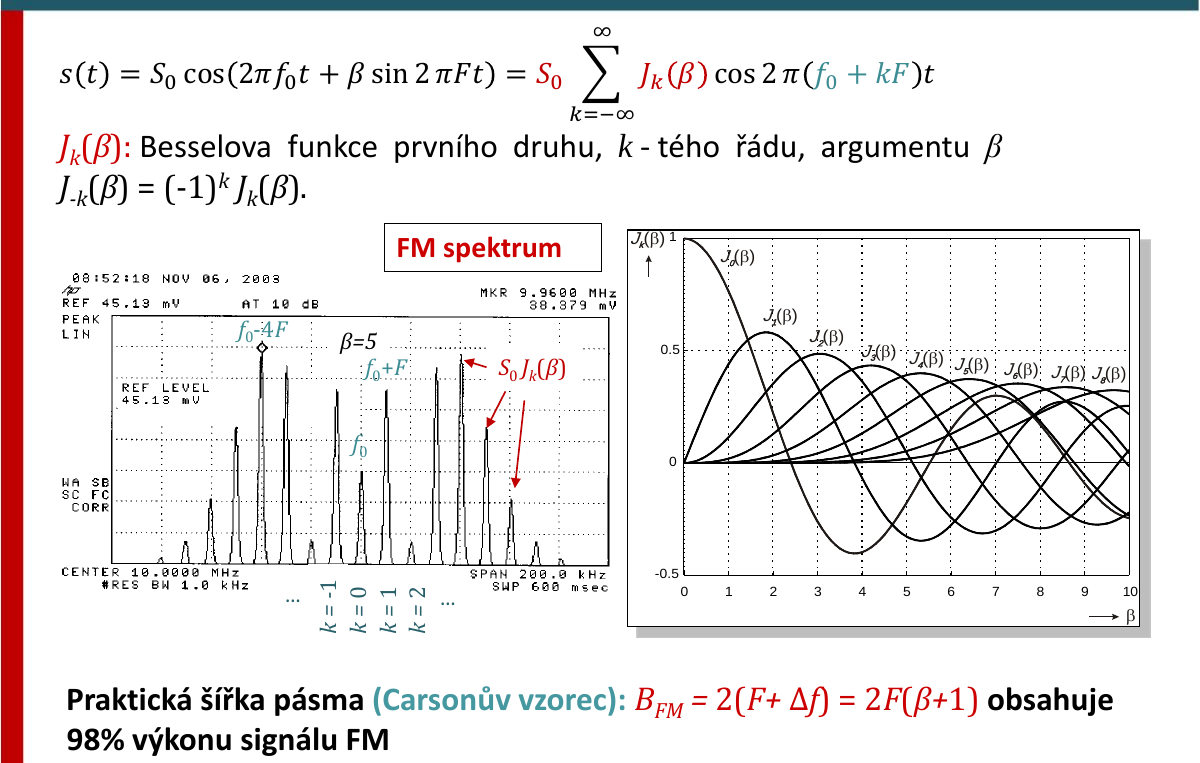
\includegraphics[width=0.92\textwidth]{Obrazky/Obrazky_KS1/fig_fm_spektrum.png}
    \caption{Vľavo: reálne FM spektrum namerané spektrálnym analyzátorom
    ($f_c = 10\,\mathrm{MHz}$, $F = 10\,\mathrm{kHz}$, $\beta = 5$). Spektrálne
    čiary sú rozmiestnené po $F$ okolo nosnej $f_0$ a ich amplitúdy sú dané
    Besselovými funkciami $S_0 J_k(\beta)$. Vpravo: priebeh Besselových funkcií
    prvého druhu $J_k(\beta)$ pre rôzne rády $k$ -- určujú výkony jednotlivých
    spektrálnych zložiek FM signálu. Carsonovo pravidlo: $B_{FM} = 2(F + \Delta f)$
    zahŕňa 98\,\% výkonu signálu.}
    \label{fig:fm_spektrum}
\end{figure}

\subsection{PM -- fázová modulácia (Phase Modulation)}

Okamžitá fáza nosnej je lineárnou funkciou modulačného signálu. FM a PM sú si
vzájomne príbuzné: FM zo signálu PM sa získa zaradením integrátora pred PM
modulátor a naopak.

\section{Digitálne modulácie v prenesenom pásme}

Pri digitálnych moduláciách nosná nadobúda diskrétne stavy zodpovedajúce
prenášaným symbolom. Počet stavov $M = 2^n$ určuje počet bitov na symbol $n$.
Vyšší počet stavov zvyšuje spektrálnu efektívnosť [bit/s/Hz], ale znižuje odolnosť
voči šumu -- body konštelačného diagramu sú si bližšie.

\subsection{BPSK a QPSK -- fázové kľúčovanie}

\textbf{BPSK} (Binary Phase Shift Keying -- binárne fázové kľúčovanie): $M = 2$
fázové stavy (0° a 180°), 1 bit/symbol. Najvyššia odolnosť voči šumu spomedzi
PSK modulácií. Používa sa pri nízkych hodnotách $E_b/N_0$ (satelitné spoje, GPS --
Global Positioning System).

\textbf{QPSK} (Quadrature Phase Shift Keying -- kvadratúrne fázové kľúčovanie):
$M = 4$ fázové stavy, 2 bity/symbol. Pri rovnakej šírke pásma ako BPSK prenesie
dvojnásobok dát. Konštelačný diagram: 4 body v rohoch štvorca.

\textbf{$\pi/4$-DQPSK} (Differential Quadrature PSK -- diferenčné QPSK):
diferenčná varianta QPSK, kde sa prenáša zmena fázy oproti predchádzajúcemu
symbolu (nie absolútna fáza). Umožňuje nekoherentnú demoduláciu.
Používa sa v systéme GSM EDGE (Enhanced Data rates for GSM Evolution).

\textbf{8PSK} (8 Phase Shift Keying): $M = 8$ fázových stavov, 3 bity/symbol.
Dobrá spektrálna účinnosť (teoreticky 3\,bit/s/Hz). Problém s obnovením nosnej
(neistota $\pm\pi/8$). Používa sa v GSM EDGE.

\begin{figure}[H]
    \centering
    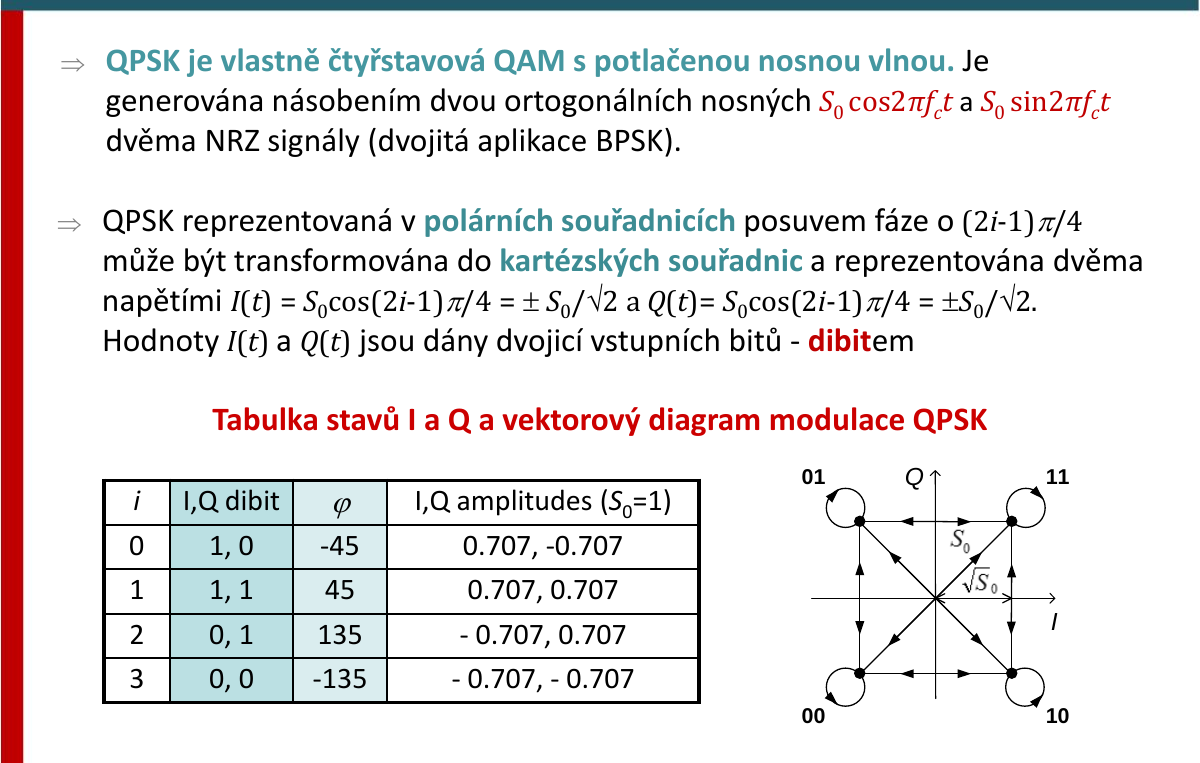
\includegraphics[width=0.82\textwidth]{Obrazky/Obrazky_KS1/fig_qpsk_konstelacia.png}
    \caption{Tabulka stavov I a Q a konštelačný (vektorový) diagram QPSK.
    Nosná nadobúda 4 fázové stavy $\pm 45°$ a $\pm 135°$. Každý stav zodpovedá
    jednému dibitu (dvojici bitov). QPSK je štvorstavová QAM s potlačenou
    nosnou -- generuje sa násobením dvoch ortogonálnych nosných ($\cos$ a $\sin$)
    dvoma NRZ (Non-Return-to-Zero) signálmi I a Q.}
    \label{fig:qpsk_konstelacia}
\end{figure}

\subsection{M-QAM -- kvadratúrna amplitúdová modulácia (Quadrature Amplitude Modulation)}

Informácia je zakódovaná súčasne v amplitúde aj fáze nosnej -- body konštelačného
diagramu tvoria pravouhlú mriežku. Pri vyššom $M$ sa zvyšuje spektrálna
efektívnosť, ale klesá odolnosť voči šumu.

\begin{itemize}
    \item 16-QAM: mriežka 4$\times$4, 4 bity/symbol -- DVB-T (Digital Video
        Broadcasting -- Terrestrial), Wi-Fi
    \item 64-QAM: mriežka 8$\times$8, 6 bitov/symbol -- káblová TV DVB-C
        (Digital Video Broadcasting -- Cable)
    \item 256-QAM: 8 bitov/symbol -- vyžaduje vysoký odstup signál/šum
\end{itemize}

\subsection{MSK a GMSK -- kmitočtové kľúčovanie so spojitou fázou}

\textbf{MSK} (Minimum Shift Keying -- kľúčovanie s minimálnym zdvihom) je členem
skupiny modulácií FSK so spojitou fázou CPFSK (Continuous Phase FSK). Pri zmene
signalizačných kmitočtov je zabezpečená plynulá zmena fázy -- bez fázových skokov.
Index modulácie $\beta = 0{,}5$ -- ide o minimálny zdvih, pri ktorom sú oba nosné
kmitočty ešte ortogonálne. Vlastnosti: možnosť nekoherentnej demodulácie, dobrá
výkonová a spektrálna účinnosť.

\textbf{GMSK} (Gaussian Minimum Shift Keying -- MSK s Gaussovým filtrom): pred
modulátor MSK je zaradená Gaussovská dolná priepusť GLPF (Gaussian Low Pass Filter).
Tá kmitočtovo obmedzí spektrum klíčovacieho signálu, čím sa výrazne potlačia
postranné laloky kmitočtového spektra modulovaného signálu. Výsledný signál GMSK
nemusí byť ďalej filtrovaný. Používa sa v GSM.

\begin{figure}[H]
    \centering
    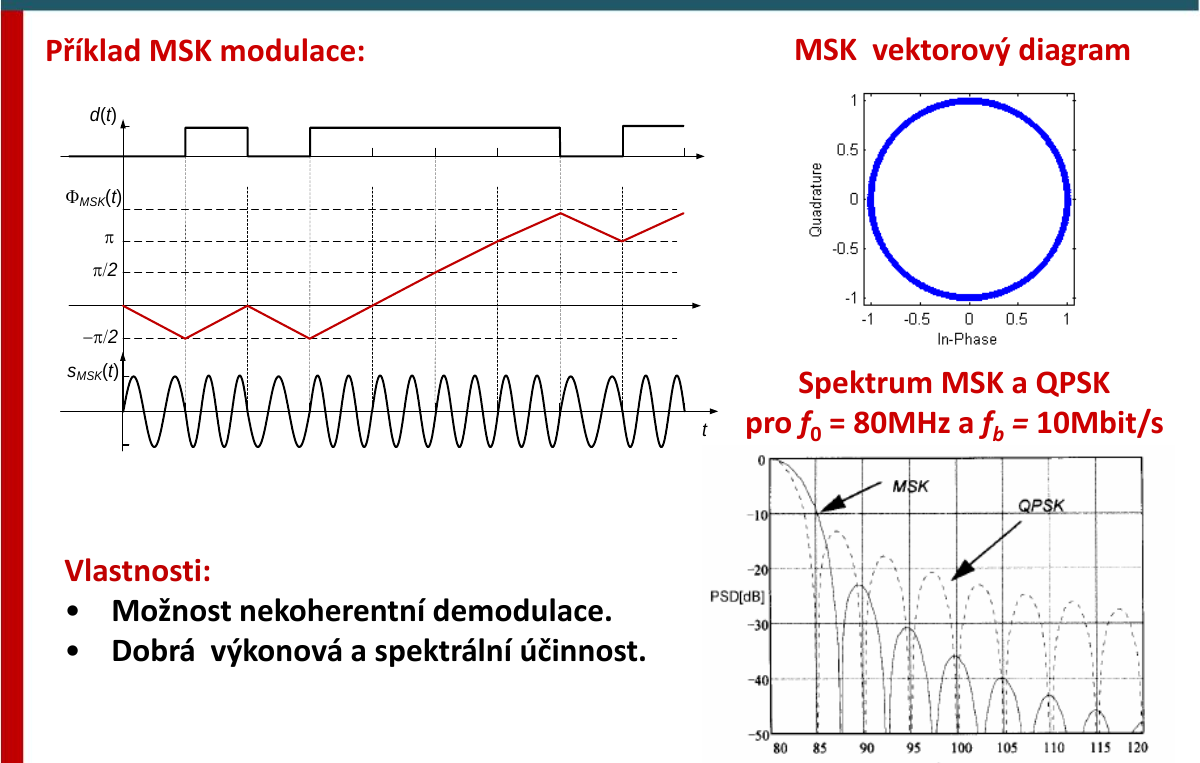
\includegraphics[width=0.90\textwidth]{Obrazky/Obrazky_KS1/fig_msk_prubehy.png}
    \caption{MSK -- príklad modulácie. Vľavo hore: dátový signál $d(t)$;
    uprostred: fázová mriež $\Phi_{MSK}(t)$ -- fáza rastie alebo klesá lineárne
    o $\pm\pi/2$ počas každej bitovej periódy $T_b$, čo zabezpečuje plynulú spojitú
    fázu; dole: výsledný MSK signál $s_{MSK}(t)$ bez fázových skokov.
    Vpravo hore: kruhový konštelačný diagram MSK (konštantná obálka).
    Vpravo dole: porovnanie spektier MSK a QPSK -- MSK má užšie hlavné laloky
    a rýchlejší pokles postranných lalokov.}
    \label{fig:msk_prubehy}
\end{figure}

\begin{figure}[H]
    \centering
    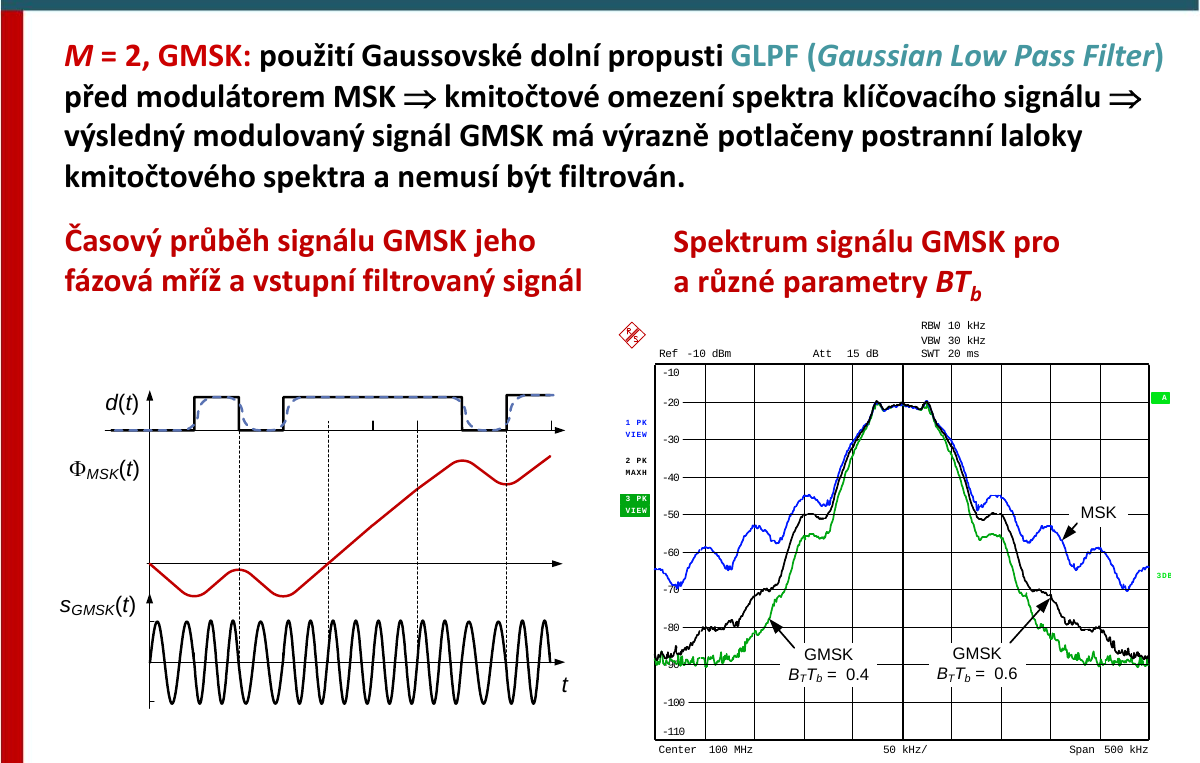
\includegraphics[width=0.90\textwidth]{Obrazky/Obrazky_KS1/fig_gmsk_spektrum.png}
    \caption{GMSK -- porovnanie s MSK. Vľavo: časový priebeh dátového signálu
    $d(t)$, fázovej mriže $\Phi_{MSK}(t)$ a výsledného GMSK signálu $s_{GMSK}(t)$ --
    Gaussovský filter zaobli ostré hrany fázovej mriže. Vpravo: skutočné spektrá
    namerané spektrálnym analyzátorom pre MSK (čierna) a GMSK s parametrami
    $BT_b = 0{,}4$ (modrá) a $BT_b = 0{,}6$ (zelená) -- GMSK má výrazne
    potlačené postranné laloky, čo znižuje medzikanálové interferencie.}
    \label{fig:gmsk_spektrum}
\end{figure}

%%%%%%%%%%%%%%%%%%%%%%%%%%%%%%%%%%%%%%%%%%%%%%%%%%%
\chapter{Synchronizácia}
%%%%%%%%%%%%%%%%%%%%%%%%%%%%%%%%%%%%%%%%%%%%%%%%%%%

\section{Prečo synchronizácia?}

Synchronizácia je neoddeliteľnou súčasťou každého digitálneho komunikačného
systému. Prijímač potrebuje poznať:
\begin{enumerate}
    \item \textbf{Presný kmitočet a fázu nosnej vlny} -- pri koherentnej demodulácii
        musí lokálne generovaná referenčná nosná byť v kmitočtovej a fázovej zhode
        s nosnou prijatého signálu. Fázová odchýlka spôsobuje rotáciu konštelačného
        diagramu a zvyšuje chybovosť.
    \item \textbf{Optimálne okamihy vzorkovania demodulovaného signálu} $T_m$ --
        vzorkovanie v okamihu maximálneho otvorenia oka minimalizuje chybovosť.
        Vzorkovanie mimo optima znižuje odstup signál/šum.
    \item \textbf{Polohu hraníc dátových rámcov} -- pri blokovom prenose a kanálovom
        kódovaní je nutné poznať začiatok každého kódového slova alebo rámca.
\end{enumerate}

\section{Diagram oka -- hodnotenie kvality synchronizácie}

\begin{figure}[H]
    \centering
    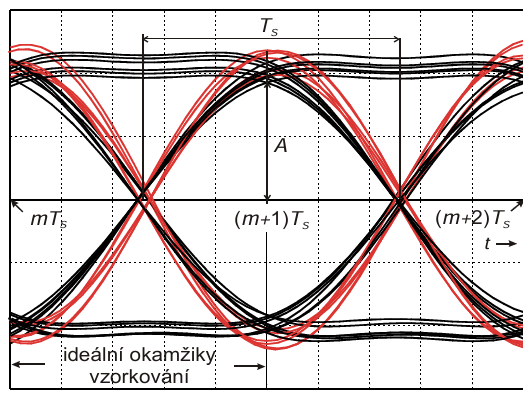
\includegraphics[width=0.55\textwidth]{Obrazky/Obrazky_KS1/fig_oko.png}
    \caption{Diagram oka vznikne superpozíciou časových priebehov demodulovaného
    signálu synchronizovaných na symbolovú periódu $T_s$. Optimálny okamih
    vzorkovania zodpovedá maximálnemu otvoreniu oka uprostred symbolovej periódy.
    Medzisymbolové interferencie ISI (Inter-Symbol Interference) a šum otvorenie
    oka zmenšujú.}
    \label{fig:oko}
\end{figure}

Diagram oka je praktický nástroj na vizuálne hodnotenie kvality digitálneho
prenosového reťazca. Úlohou obvodu obnovy časovania symbolov STR (Symbol Timing
Recovery) je nájsť a udržať okamih maximálneho otvorenia oka.

\section{PLL -- základ synchronizačných obvodov}

\textbf{PLL} (Phase-Locked Loop -- slučka fázového závěsu) je spätnoväzobný
obvod sledujúci fázu a kmitočet vstupného signálu. Tvoria ho tri základné časti:

\begin{itemize}
    \item \textbf{Fázový detektor} -- porovnáva fázy vstupného signálu $\theta_i$
        a výstupu VCO $\theta_o$; generuje chybové napätie $u_e = K_d(\theta_i - \theta_o)$
    \item \textbf{Dolná priepusť} $F(p)$ -- filtruje chybové napätie a tvaruje
        dynamiku slučky
    \item \textbf{VCO} (Voltage Controlled Oscillator -- napätím riadený oscilátor)
        -- mení okamžitý kmitočet úmerne riadiacemu napätiu: $\Delta\omega_o = K_o u_c(t)$;
        spätná väzba udržuje $\theta_e \to 0$
\end{itemize}

\begin{figure}[H]
    \centering
    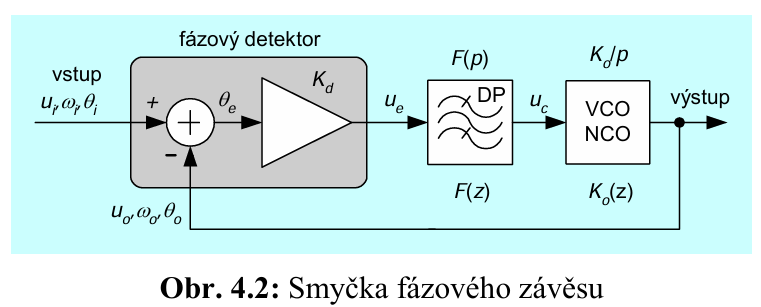
\includegraphics[width=0.75\textwidth]{Obrazky/Obrazky_KS1/fig_pll.png}
    \caption{Blokové schéma PLL. Fázový detektor generuje chybové napätie úmerné
    fázovej odchýlke. Dolná priepusť tvaruje dynamiku slučky. VCO mení okamžitý
    kmitočet úmerne riadiacemu napätiu. Spätná väzba udržuje fázovú odchýlku
    blízku nule.}
    \label{fig:pll}
\end{figure}

\textbf{Dva pracovné režimy PLL:}
\begin{itemize}
    \item \textbf{Zachytávanie} (acquisition): prechodný dej konvergencie do
        závesného stavu
    \item \textbf{Sledovanie} (tracking): ustálený závesný stav so sledovaním
        malých zmien kmitočtu a fázy
\end{itemize}

\textbf{DPLL} (Digital PLL -- číslicová slučka fázového závěsu): číslicová
implementácia -- VCO je nahradený číslicovo riadeným oscilátorom NCO (Numerically
Controlled Oscillator).

Aplikácie PLL a DPLL: obnova nosnej v systémoch s nepotlačenou nosnou, modulácia
a demodulácia FM/PM/FSK, násobenie kmitočtu, stavebný blok systémov CR (Carrier
Recovery) a STR.

\section{Obnova nosnej vlny (CR -- Carrier Recovery)}

Pri moduláciách s potlačenou nosnou (DSB-SC, BPSK, QPSK, QAM) nosná zložka
v spektre prijatého signálu chýba -- prijímač ju musí obnoviť priamo
z modulovaného signálu. Existujú dve základné metódy:

\begin{itemize}
    \item Použitie pomocných nemodulovaných \textbf{pilotných signálov}:
        TIB (Tone in Band -- tón v pásme) -- kontinuálne vysielané pomocné signály,
        alebo PSAM (Pilot Symbol-Assisted Modulation -- modulácia asistovaná
        pilotným symbolom) -- referenčné symboly vkladané do dátového toku.
        Nevýhoda: znižuje energetickú alebo kapacitívnu účinnosť systému.
    \item \textbf{Extrakcia nosnej z postranných pásiem} (s využitím PLL) --
        umocňujúca slučka (Squaring Loop) alebo Costasova slučka (Costas Loop).
\end{itemize}

\begin{figure}[H]
    \centering
    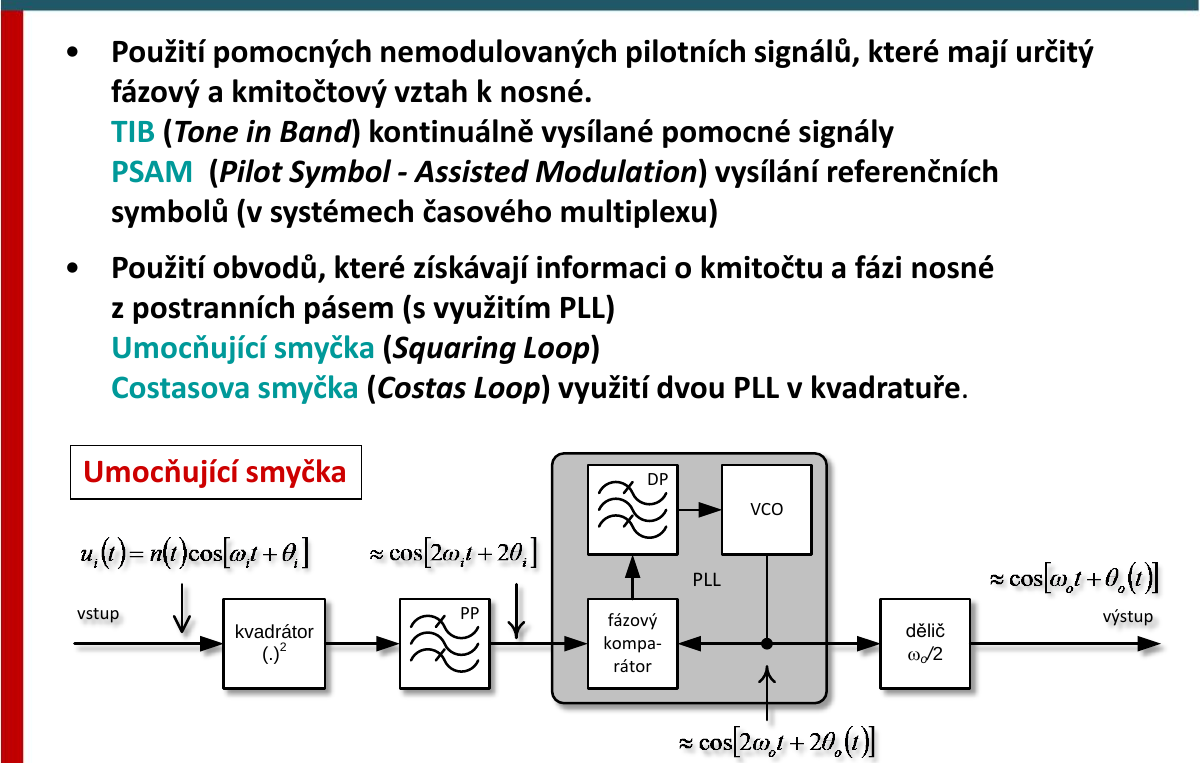
\includegraphics[width=0.90\textwidth]{Obrazky/Obrazky_KS1/fig_umocnujuca_slucka.png}
    \caption{Metódy obnovy nosnej pri potlačenej nosnej vlne. Hore: prehľad
    metód (pilotné signály TIB/PSAM, umocňujúca slučka, Costasova slučka).
    Dole: blokové schéma umocňujúcej slučky pre BPSK/DSB. Vstupný signál
    $u_i(t) = n(t)\cos[\omega_i t + \theta_i]$ sa umocní kvadrátorom $(\cdot)^2$,
    čím sa odstráni dátová modulácia a vznikne zložka na $2\omega_i$.
    Pásmová priepusť (PP) vyčlení túto zložku, slučka PLL ju sleduje a stabilizuje,
    delič kmitočtu $\omega_o/2$ obnoví nosnú na pôvodnom kmitočte $\omega_c$.}
    \label{fig:umocnujuca_slucka}
\end{figure}

\subsection{Umocňujúca slučka}

Pri BPSK signáli fázové kľúčovanie spôsobuje skoky fázy o $\pi$ -- nosnú
priamou filtráciou nemožno extrahovať. Po umocnení signálu na druhú sa fázové
kľúčovanie odstráni (keďže $m^2(t) = 1$ pre $m(t) \in \{+1,-1\}$) a vznikne
zložka na kmitočte $2f_c$, ktorú možno vyčleniť pásmovou priepusťou a sledovať
slučkou PLL. Delič kmitočtu 2 obnoví nosnú na $f_c$.

\begin{figure}[H]
    \centering
    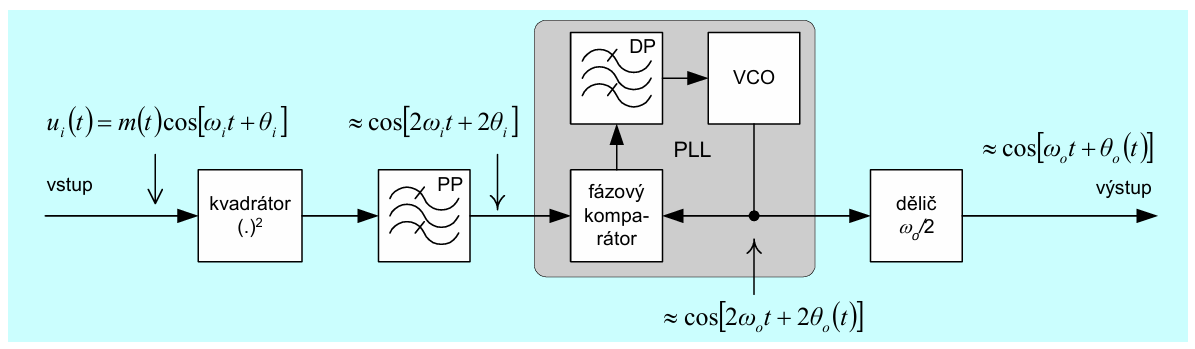
\includegraphics[width=0.80\textwidth]{Obrazky/Obrazky_KS1/fig_kvadrator.png}
    \caption{Obvod pre obnovu nosnej s kvadrátorom pre BPSK/DSB. Kvadrátor
    ($(\cdot)^2$) odstráni dátovú moduláciu. Pásmová priepusť vyčlení zložku
    na $2f_c$. PLL stabilizuje fázu. Delič kmitočtu 2 obnoví nosnú na $f_c$.}
    \label{fig:kvadrator}
\end{figure}

\subsection{Costasova slučka}

Costasova slučka vykonáva súčasne koherentnú demoduláciu aj obnovu nosnej.
Vstupný signál sa násobí dvoma kvadratúrnymi replikami výstupu VCO -- synfáznou
(vetva I -- In-phase) a kvadratúrnou (vetva Q -- Quadrature). Pri nulovej fázovej
odchýlke $\theta_e = 0$ je výstup vetvy Q nulový. Pri nenulowej $\theta_e$ sa na
vetve Q objaví nenulové napätie, ktoré -- po prechode rozhodovacím obvodom RO
(Rozhodovací Obvod) a násobiačom N3 -- tvorí chybové napätie $u_e(t) \approx
\theta_e(t)$ riadi VCO k nulovej odchýlke.

\begin{figure}[H]
    \centering
    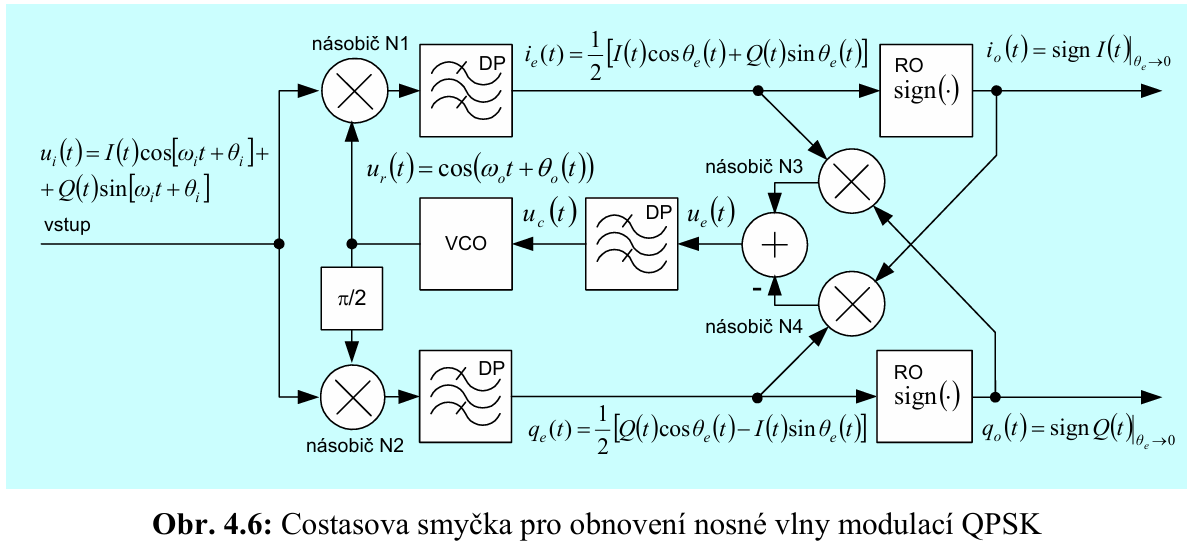
\includegraphics[width=0.85\textwidth]{Obrazky/Obrazky_KS1/fig_costas_qpsk.png}
    \caption{Costasova slučka pre QPSK. Vetvy I a Q poskytujú demodulované dátové
    signály. Rozhodovacie obvody (RO) realizujúce funkciu $\mathrm{sgn}(\cdot)$
    odstraňujú dátovú moduláciu zo spätnoväzobnej vetvy. Násobiče N3 a N4
    generujú chybové napätie pre VCO.}
    \label{fig:costas}
\end{figure}

\subsection{Slučka s rozhodovacou spätnou väzbou (DFBL -- Decision Feedback Loop)}

Chybové napätie sa generuje z korelácie odhadnutého (dekódovaného) symbolu
s oneskorením výstupu kvadratúrnej vetvy. Odhadnutý symbol je ``čistejší'' ako
surový demodulovaný signál $\Rightarrow$ nižšia fázová chyba.

\begin{figure}[H]
    \centering
    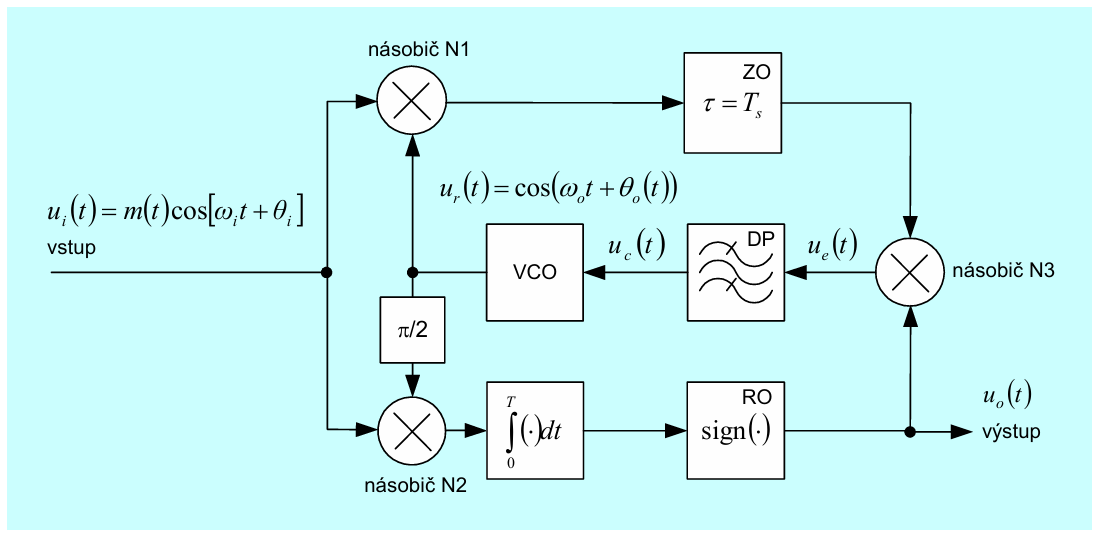
\includegraphics[width=0.80\textwidth]{Obrazky/Obrazky_KS1/fig_dfbl.png}
    \caption{Slučka DFBL pre BPSK. Prispôsobený filter (korelátor) + rozhodovací
    obvod poskytujú odhadnutý symbol. Oneskorený výstup násobiča N2 sa koreluje
    s odhadnutým symbolom (násobič N3) $\Rightarrow$ chybové napätie pre VCO.}
    \label{fig:dfbl}
\end{figure}

\section{Obnova časovania symbolov (STR -- Symbol Timing Recovery)}

Cieľom je nájsť a udržať optimálne okamihy vzorkovania demodulovaného signálu.
Rozlišujú sa dva typy metód:

\begin{itemize}
    \item \textbf{DA} (Data-Aided -- s pomocou dát): informácia o časovaní sa
        prenáša spolu s dátami -- buď pomocou kmitočtového multiplexu (pilotný
        signál na pomocnej nosnej) alebo časovým multiplexom (známa symbolová
        postupnosť vložená do dátového toku).
    \item \textbf{NDA} (Non Data-Aided -- bez pomocných dát): informácia
        o vzorkovacích okamihoch sa extrahuje priamo z dátového prúdu -- nevyžaduje
        špeciálny kanál.
\end{itemize}

\subsection{Early-Late synchronizátor}

Najrozšírenejší STR obvod so spätnou väzbou. Porovnáva energie signálu integrovaného
v dvoch susedných intervaloch:

\begin{itemize}
    \item \textbf{Early integrátor}: integruje prvú polovicu symbolovej periódy
        (pred odhadovaným optimom)
    \item \textbf{Late integrátor}: integruje druhú polovicu symbolovej periódy
        (za odhadovaným optimom)
\end{itemize}

Pri správnej synchronizácii sú absolútne hodnoty výstupov oboch integrátorov
zhodné a chybové napätie $u_e = |u_E| - |u_L| = 0$. Pri časovej odchýlke je
energia rozdelená nesymetricky -- chybové napätie koriguje kmitočet VCO v správnom
smere.

\section{Rámcová synchronizácia (FS -- Frame Synchronization)}

Dátový tok je organizovaný do rámcov pevnej štruktúry. Na identifikáciu začiatku
rámca sa do hlavičky vkladá \textbf{synchronizačné kódové slovo} so špeciálnymi
korelačnými vlastnosťami.

\textbf{Barkerove postupnosti} sú binárne postupnosti s výnimočnými korelačnými
vlastnosťami: autokorelačná funkcia má ostrý vrchol $C_0 = N$ a všetky
mimostredové korelačné koeficienty splňujú $|C_k| \leq 1$ pre $k \neq 0$.
Prijímač realizuje korelátor (prispôsobený filter) -- pri zarovnaní s kódovým
slovom vznikne výrazný korelačný vrchol jednoznačne indikujúci začiatok rámca.

Existuje 10 Barkerových postupností s dĺžkou $N \leq 13$. Pre dlhšie rámce
sa používajú počítačom nájdené postupnosti väčšej dĺžky (Newmanove, Linderove).

Systém je charakterizovaný dvoma pravdepodobnosťami, ktoré je nutné minimalizovať:
$P_m$ (chýbajúca detekcia -- miss detection) a $P_{fa}$ (plané poplach -- false alarm).
Ich požiadavky sú protichodné -- väčšia dĺžka kódového slova $N$ znižuje $P_m$,
ale zvyšuje $P_{fa}$.

\section{Sieťová synchronizácia}

V systémoch s časovým multiplexom TDMA (Time Division Multiple Access -- viacnásobný
prístup s časovým delením), kde viac terminálov zdieľa jeden kanál s centrálnym
uzlom (napr. satelitná stanica), musí každý terminál \textbf{predkorigovať časovanie
svojho vysielača}, aby jeho signál dorazil do uzla v pridelenom časovom slote.
Rozlišujeme:

\begin{itemize}
    \item \textbf{Otvorená slučka} (open-loop): terminál vypočíta časovú
        predkorekciu $d/c$ z odhadnutej vzdialenosti $d$ k uzlu. Rýchle uvedenie
        do prevádzky, ale presnosť je obmedzená chybami odhadu vzdialenosti
        a nestabilitou časových normálov. Vhodné pre geometricky stabilné
        systémy pracujúce dlhodobo.
    \item \textbf{Uzavretá slučka} (closed-loop): uzol meria časové odchýlky
        príchodzích signálov a posiela korekčné informácie späť terminálom.
        Vyššia presnosť, ale vyžaduje spätný kanál. Výhodné najmä pri TDMA,
        kde je výpočtová kapacita pre určenie synchronizačných chýb zdieľaná
        všetkými terminálmi.
\end{itemize}